\documentclass{article}[10pt]
\usepackage[utf8]{inputenc}
\usepackage[margin=1in]{geometry}
\usepackage{amsmath}
\usepackage{amssymb}
\usepackage{amsthm}
\usepackage{tikz}
\usepackage{graphicx}
\usepackage{wrapfig}
\usepackage{float}
\usepackage{siunitx}
\graphicspath{ {Images/} }



\begin{document}
\section{Wave-particle duality}
TODO:\@ Find a way to make a scheme like the one on my notes. All it does is say
that the atomic number is the number of electrons which is equals to the number
of protons, and that the mass is the protons plus the neutrons. 

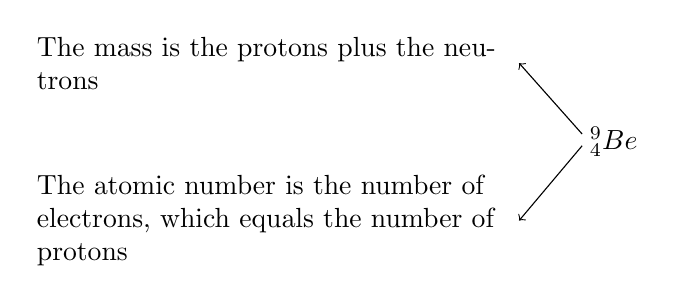
\begin{tikzpicture}
  \draw (0.2,0) node {${}^9_4Be$};
  \draw [left, text width=6cm](-1,1) node {The mass is the protons plus the neutrons};
  \draw [left, text width=6cm](-1,-1) node {The atomic number is the number of electrons, which equals the number of protons};
  \draw [->] (-0.2,-0.05) -- (-1,-1);
  \draw [->] (-0.2,0.1) -- (-1,1);
\end{tikzpicture}

\subsection{Characteristics of a Wave}
\begin{itemize}
    \item Wave Length ($\lambda$) --- Distance between two consecutive points of
          equal vibrational phase.

          TODO:\@ Add pretty image of wave showing $\lambda$
          \begin{figure}[H]
          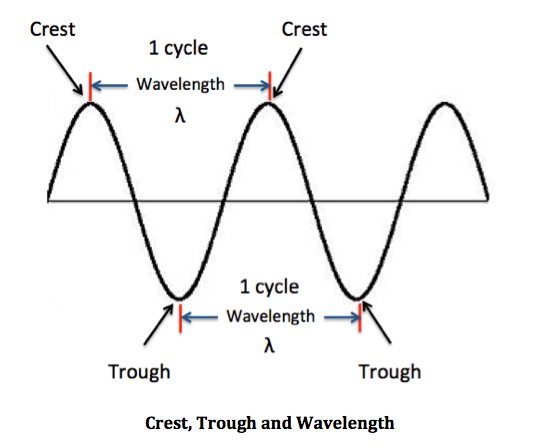
\includegraphics[scale=0.5]{lambdawave}
          \end{figure}

          \begin{align*}
              1\si{\micro\metre} = \num{e-6}\si{\metre} \\[0.5em]
              1\si{\nano\metre} = \num{e-9}\si{\metre}  \\[0.5em]
              1\si{\angstrom} = \num{e-10}\si{\metre}   \\[0.5em]
              1\si{\pico\metre} = \num{e-12}\si{\metre} \\[0.5em]
          \end{align*}
    \item Frequency ($\nu$) --- Number of vibrations or complete cycles per
          unit of time.
          \begin{align*}
              1\si{\mega\hertz} = \num{e6}\si{\hertz} \\[0.5em]
              1\si{\giga\hertz} = \num{e9}\si{\hertz} \\[0.5em]
              1\si{\tera\hertz} = \num{e13}\si{\hertz} \\[0.5em]              
          \end{align*}
          TODO:\@ Finish these
    \item Period ($\tau$) --- Duration of a cycle $V=\frac{1}{T}$
\end{itemize}

\end{document}
